%!TEX root = m392c_EHT_notes.tex

\begin{quote}\textit{
	``Smith's theorem was proven by Smith, hence the name.''
}\end{quote}
% Today I was running about two minutes late. Sorry, everybody! (What I missed: Andrew discussed holding a ``Q and
% A'' session next week on a weeknight, perhaps with pizza. If you're interested in this, email him to let him know
% which nights work for you.)
%
Another consequence of Elmendorf's theorem (\cref{revElmen}) is that presheaves on the orbit category that are
valued in abelian groups are Eilenberg-Mac Lane $G$-spaces. Homotopy classes of maps into these $G$-spaces gives
what's known as Bredon cohomology; we'll introduce this and compute several examples.\index{Elmendorf's theorem}
\begin{defn}
Let $G$ be a finite group, A \term{coefficient system} is a presheaf $X\in\Fun(\sO_G\op, \Ab)$
\end{defn}
Elmendorf's theorem says that for any coefficient system, we have an Eilenberg-Mac Lane $G$-space. You could say
here that (Bredon) cohomology is completely determined: cohomology is the things represented by Eilenberg-Mac Lane
spaces. But it will be good to see it explicitly. Bredon cohomology is explicit, but there are serious drawbacks:
it has poor formal properties, and you need a lot of geometric insight to compute things. We'll later see that this
abelian category (meaning we can do homological algebra) is the wrong one; it produces a $\Z$-graded cohomology
theory (or rather, one graded on subgroups of $\Z$); this will be the wrong answer, especially if you want Poincaré
duality, and the right answer uses a grading by the representation ring. But we'll get there.\index{Eilenberg-Mac
Lane space}\index{Poincaré duality}
\begin{rem}
If $G$ is a compact Lie group, the proper definition of a coefficient system is an $\Ab$-valued presheaf on
$h\sO_G$, the homotopy category of the orbit category. (For finite groups these definitions coincide.) In other
words, given $G$ a compact Lie group and a family of subgroups $\sF$ of $G$, the homotopy orbit category $h\sO_G$
has objects $G/H$, where $H \in \sF$, and has morphisms the homotopy classes of maps $G/H \to G/K$.\index{homotopy
category!of the orbit category}
\end{rem}
% TODO: if you put this example inside the remark, it's typeset wrong.
\begin{exm}
Let us consider $h\sO_{S^1}$, the homotopy orbit category for $S^1$ with $\sF$ the family of finite subgroups of
$S^1$.

We first consider the orbit category $\sO_{S^1}$. Since $S^1$ is abelian, we have a morphism $G/H \to G/K$
if and only if $H \subseteq K$. In fact,
	\[\Hom_{\sO_{S^1}}(G/H, G/K) =
	\begin{cases}
	G/K, &\text{if }H \subseteq K\\
	0, &\text{otherwise.}
	\end{cases}\]
The homotopy orbit category $h\sO_{S^1}$ is not too much more difficult: since $S^1$ is connected, if $H \subseteq
K$, then all maps $G/H \to G/K$ are homotopic (they are maps of circles of the same degree). Hence, we have
	\[\Hom_{h\sO_{S^1}}(G/H, G/K) = \begin{cases}
	1, &\text{if } H \subseteq K\\
	0, &\text{otherwise.}
	\end{cases} \qedhere\]
\end{exm}
Coefficient systems have an important role in Bredon cohomology, which is calculated with coefficients in a
coefficient system, and whose construction makes use of a chain complex of coefficient systems. In this way,
coefficient systems play the part in Bredon cohomology that abelian groups do in CW cohomology. Indeed, coefficient
systems form an abelian category; it may be helpful to think of it as the category of ``right $\sO_G$-modules,''
even if that isn't literally true.

Here are some examples of coefficient systems (which are often denoted with underlines).
\begin{comp}{exm}{enumerate}
	\item $\underline \Z$ will denote the \term{constant coefficient system} with coefficients in $\Z$, i.e.\ the
	functor which sends all objects to $\Z$ and all morphisms to $\id_\Z$. You can replace $\Z$ with your favorite
	abelian group.
	\item For a $G$-space $X$, the coefficient system $\underline\pi_n(X)$ ($n\ge 2$) sends $G/H\mapsto\set{\pi_nX^H}$. This is an example of
	a general formula: given a functor $\Top\to\Ab$, we can compose to obtain a map $\Fun(\sO_G\op,
	\Top)\to\Fun(\sO_G\op, \Ab)$.
	\item In the same way, $\underline H_n(X)$ sends $G/H\mapsto\set{H_n(X^H;\Z)}$.\qedhere
\end{comp}
We will now define Bredon cohomology, due to Bredon~\cite{Bredon}, which is the analogue of CW cohomology for
$G$-CW complexes.
\begin{defn}
We first define a chain complex of coefficient systems $\underline C_\bullet(X)$, which is the analogue of the CW
chain complex. It sends an orbit $G/H$ to the CW chains of $X^H$.\footnote{This requires knowing how to obtain a CW
structure on $X^H$ given a $G$-CW structure on $X$. If $G$ is finite, this is easy to see; for general compact Lie
groups, though, this requires a triangulation argument. One wants the resulting coefficient system to be
independent of the choice of triangulation, but as in the nonequivariant case, this is proven via an axiomatic
characterization of cohomology.}

Let $X$ be a $G$-CW complex and $X_n$ denote its $n$-skeleton. Let
\[\underline C_n(X) \coloneqq \underline H_n(X_n, X_{n-1};\Z),\]
i.e.\ the coefficient system sending $G/H\mapsto H_n((X^H)_n, (X^H)_{n-1};\Z) = C_n^{\text{CW}}(X^H)$. The
differential at $G/H$ is the CW chain complex differential for $X^H$, i.e.\ the connecting morphism in the long
exact sequence of the triple $((X^H)_n, (X^H)_{n-1}, (X^H)_{n-2})$. One should check that this commutes with the
bonding maps for $\underline C_n(X)$, but it does, so this works.
\end{defn}
%The \term{Bredon cohomology} with coefficients in a coefficient system $M$ is
%\[H^n_G(X;M) \coloneqq H^n\paren{\Hom_{\Fun(\sO_G\op, \Ab)}(\underline C_\bullet(X), M)}.\]
%\end{defn}
%
%We'll continue to discuss Bredon cohomology next lecture, and introduce an axiomatic viewpoint. This is basic and
%fundamental, but not too relevant to the rest of the class. It's also good to calculate; there are surprisingly few
%examples out in the world.
%Today we'll continue Bredon cohomology, and state a version of the Eilenberg-Steenrod axioms that characterize it.
%Then, we'll turn to the circle of ideas around Smith theory, including the Sullivan conjecture (which we won't
%prove, because it's hard). Smith theory is about when one can recover $H_*(X^G)$ from algebraic information derived
%from the $G$-action on $X$.
% Let's recall the definition of Bredon cohomology from last time: if $X$ is a $G$-CW complex, let $\underline
% C_*(X)$ denote the chain complex of coefficient systems (i.e.\ functors $\sO_G\op\to\Ab$)
% \[\underline C_n(X)(G/H)\coloneqq H_n((X^H)_n, (X^H)_{n-1}; \Z).\]
% The differential $\partial\colon\underline C_n(X)\to\underline C_{n-1}(X)$ is the same as in CW cohomology, the
% connecting morphism in the long exact sequence for the triple $(X_n, X_{n-1}, X_{n-2})$; that $\partial^2 = 0$ is
% something you have to check, though it's not very difficult.
Using this chain complex, we define Bredon homology and cohomology.
\begin{comp}{defn}{itemize}
	\item The \term{Bredon cohomology} with coefficients in a coefficient system $M$ is
	\[H_G^n(X;M) \coloneqq H^n(\Hom_{\Fun(\sO_G\op, \Ab)}(\underline C_*(X), M)).\]
	That is, we take the chains on $X$ and compute the maps into $M$; since $\Fun(\sO_G\op,\Ab)$ is an abelian
	category, this is a cochain complex of abelian groups, and we can take its homology to obtain a sequence of
	abelian groups.
	\item For homology to be a covariant functor, we need the coefficient system $M$ to be a functor $\sO_G\to\Ab$
	rather than $\sO_G\op\to\Ab$ (e.g.\ $\underline H^*(X)$ for a $G$-space $X$, which sends
	$G/H\mapsto\set{H^n(X^H)}$).\footnote{Would it be appropriate to call such a functor an ``efficient system?''}
	With $M$ such a coefficient system, the \term{Bredon homology} with coefficients in $M$ is
	\[H_n^G(X; M) \coloneqq H_n(\underline C_n(X)\otimes_{\sO_G} M).\]
	By this tensor product, we mean a coend:\index{coend}
	\begin{align*}
	\underline C_n(X)\otimes_{\sO_G} M &= \int^{G/H\in \sO_G} \underline C_n(X)(G/H)\otimes M(G/H)\\
	&= \bigoplus_{G/H} {\underline C_n(X)(G/H)\otimes M(G/H)} \mathbin/ {\mathord\sim},
	\end{align*}
	where if $f\in\Map_{\sO_G}(G/H, G/K)$, $(f^*y, z)\sim (y, f_*z)$.\footnote{Tensor products are particular
	instances of coends; instead of inducing an equivalence $mr\otimes n\sim m\otimes rn$, you flip a map across
	the two objects. One might write $y\cdot f$ for $f^* y$ and $f\cdot z$ for $f_* z$ to emphasize this point of
	view.}
\end{comp}
The whole philosophy of Bredon (co)homology is to understand equivariant cohomology and homology through the
fixed-point sets and the lattice of subgroups of $G$.

Now we'll compute some simple examples of Bredon homology and cohomology over $C_2$. Its orbit category is simple:
\begin{equation}
\label{C2orbit}
\gathxy{
	C_2/e\ar[d]\ar@(ul, ur)_{}\\
	C_2/C_2.
}
\end{equation}
The map $C_2/e\to C_2/C_2$ crushes $C_2/e$ to a point, and the map $C_2/e\to C_2/e$ exchanges the two
points.\index{orbit category!of $C_2$}
\begin{exm}
\label{2sigmaBC}
Let $C_2$ act on $S^2$ by rotation by $\pi$. We'll compute the Bredon cohomology of this $C_2$-space with
coefficients in $\underline\Z$.\index{sign representation}
\begin{ex}
If $\sigma\colon C_2\to\GL_1(\R)$ denotes the sign representation, verify this $C_2$-action on $S^2$ makes it into
the representation sphere $S^{2\sigma}$.
\end{ex}
To compute the Bredon cohomology of $S^{2\sigma}$, we first need a $C_2$-CW structure on it. We've already computed
one in \cref{S2sigmaCW}: the two fixed points are two $0$-cells $C_2/C_2\times D^0$, a great circle through them is
the single $1$-cell $C_2/e\times D^1$, and the two hemispheres are the single $2$-cell $C_2/e\times D^2$. See
\cref{S2CWrotation} for a picture.
\begin{figure}[h!]
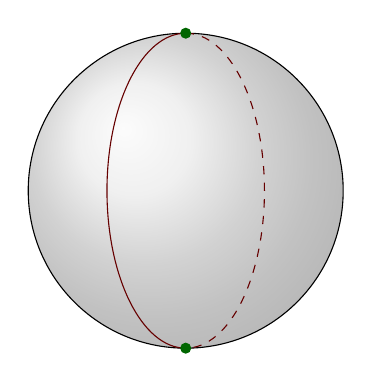
\begin{tikzpicture}
  \shade[ball color = gray!40, opacity = 0.4] (0,0) circle (2cm);
  \draw (0,0) circle (2cm);
  \draw[red!40!black] (0,2) arc (90:270:1cm and 2cm);
  \draw[dashed, red!40!black] (0,2) arc (90:-90:1cm and 2cm);
  \fill[green!40!black, fill=green!40!black] (0,2) circle (2pt);
  \fill[green!40!black, fill=green!40!black] (0,-2) circle (2pt);
\end{tikzpicture}
\caption{A $C_2$-CW structure on $S^{2\sigma}$, the $2$-sphere with a $C_2$-action by rotation through $180^\circ$.
The two green dots are the two $0$-cells $C_2/C_2\times D^0$; the red circle is the single $1$-cell $C_2/e\times
D^1$, and the gray hemispheres are the single $2$-cell $C_2/e\times D^2$.}
\label{S2CWrotation}
\end{figure}

Next we compute $\underline C_*(S^{2\sigma})$. A coefficient system is determined by a map $M_1\to M_2$ and an
involution on $M_2$. In our case, $\underline C_k(X)(C_2/e) = \Z\oplus\Z$ for $k = 0,1,2$, and the involution flips
the two factors.  Therefore we obtain a chain complex of coefficient systems which is
\[
\shortexact[f_1][f_2]{\Z\oplus\Z}{\Z\oplus\Z}{\Z\oplus\Z}{}
\]
at $C_2/e$ and
\begin{equation}
\label{C_2/C_2}
\shortexact{0}{0}{\Z\oplus\Z}{}
\end{equation}
at $C_2/C_2$.
Next we need to determine the differentials.  By definition, these are determined by the cellular boundary maps, i.e.\ the attaching maps. Let $(x,y)$ denote the standard basis of $\Z\oplus\Z$.
\begin{itemize}
	\item $f_1$ sends $(x,y)\mapsto (x+y, x+y)$.
	\item $f_2$ sends $(x,y)\mapsto (x-y, y-x)$, 
\end{itemize}

\iffalse
In terms of matrices, the differentials are given by
\[\xymatrix{
	0 \ar[r] & \Z\oplus\Z \ar[r]^-{\text{\tiny$\matr 1{-1}1{-1}$}} & \Z\oplus\Z \ar[r]^-{\text{\tiny$\matr 1{-1}{-1}1$}} & \Z\oplus\Z \ar[r] & 0
}\]
\fi

Next, we compute the $\Hom$ from this coefficient system to the constant coefficient system $\underline\Z$.  These groups are evidently determined by what happens at the $C_2/e$ spot.  For the first two terms, we are looking at maps $\Z \oplus \Z \to \Z$ that are equivariant (where $g \in C_2$ acts by transposition on the left and trivially on the right).  Such a map is determined by where it sends $(1,0)$, and so these two terms are isomorphic to $\Z$.  The last term is simply all homomorphisms $\Z \oplus \Z \to \Z \oplus \Z$, which is isomorphic to $\Z \oplus \Z$.
Therefore, we have the cochain complex
\[
\shortexact{\Z \oplus \Z}{\Z}{\Z}.
\]
Computing the differentials, we find that the first map is $(a,b) \mapsto a+b$ and the second map is $0$.

Taking the cohomology of this complex then produces
\[H^n(S^{2\sigma};\underline\Z) = \begin{cases}
	\Z, & n = 0, 2\\
	0, &\text{otherwise.}
\end{cases}\]
Now, we'll compute the Bredon homology of $S^{2\sigma}$, again with coefficients in the constant functor valued in
$\Z$. First we need to compute the tensor product $\underline C_\bullet(X)\otimes_{\sO_{C_2}}\underline\Z$:


%Let $C_2$ act on the sphere by rotation by $\pi$, as before, with the same $C_2$-CW structure. Thus $\underline
%C_\bullet(S^2)$ is the same, and we need to tensor it with $\underline\Z$. The result is the chain complex
\[\xymatrix{
	\Z^2 & \Z^2/\ang{[1,-1]}\ar[l]_-{\begin{psmallmatrix*}[r]1\\-1\end{psmallmatrix*}} & \Z^2/\ang{[1,-1]}.\ar[l]_0
}\]
Hence the Bredon homology of $S^{2\sigma}$ is
\[H^{C_2}_k(S^{2\sigma}; \underline\Z) = \begin{cases}
	\Z^2, &k = 0\\
	\Z, &k = 2\\
	0, &\text{otherwise.}
\end{cases}\]
\TODO: shouldn't it be $\Z$, $0$, $\Z$?
\end{exm}
\begin{rem}
We're used to reading off properties of a space from its cohomology, and this is still true here, if harder. For
example, $H^0$ tells us the number of connected components of $S^2/C_2$.
\end{rem}
\begin{ex}
Generalize \cref{2sigmaBC} to $S^{n\sigma}$, the $n$-sphere with a $C_2$-action given by a half-turn.
\end{ex}
\begin{exm}
Let $C_2$ act on $S^2$ by the antipodal action.\index{antipodal map}
\begin{ex}
Identify this action with that of the unit sphere $S(3\sigma)$ in $3\sigma$ (i.e.\ a direct sum of three copies of
the sign representation).\index{sign representation}
\end{ex}

We get a $C_2$-CW structure of \TODO. We'll again compute the
Bredon cohomology of $S^2$ with coefficients in $\underline\Z$.

The chain complex $\underline C_\bullet(S(3\sigma))$ is
\[\xymatrix@C=1.5cm{
	\Z^2\ar@(ur,ul)_{\begin{psmallmatrix}0&1\\1&0\end{psmallmatrix}} &
	\Z^2\ar[l]_{\begin{psmallmatrix*}[r]1&-1\\-1&1\end{psmallmatrix*}}
	\ar@(ur,ul)_{\begin{psmallmatrix}0&1\\1&0\end{psmallmatrix}} &
	\Z^2\ar[l]_{\begin{psmallmatrix}1&1\\1&1\end{psmallmatrix}}
	\ar@(ur,ul)_{\begin{psmallmatrix}0&1\\1&0\end{psmallmatrix}}\\
	0\ar[u] & 0\ar[u]\ar[l] & 0.\ar[u]\ar[l]
}\]
Now we need to take $\Hom(\bl,\underline\Z)$. In each degree we get a one-dimensional space of maps generated by
$(1,1)$. The differential $\partial\colon C^0\to C^1$ sends
\[(1,1)\mapsto (1,1)\circ\begin{pmatrix*}[r]1 & -1\\-1 & 1\end{pmatrix*} = \begin{pmatrix}0\\0\end{pmatrix},\]
and the differential $\partial\colon C^1\to C^2$ sends
\[(1,1)\mapsto (1,1)\circ\begin{pmatrix*}[r]1 & 1\\1 & 1\end{pmatrix*} = \begin{pmatrix}2\\2\end{pmatrix}.\]
Hence the cochain complex is
\[\xymatrix{
	\Z\ar[r]^0 & \Z\ar[r]^2 & \Z,
}\]
so the Bredon cohomology is
\[H_{C_2}^k(S(3\sigma);\underline\Z) = \begin{cases}
	\Z, &k = 0\\
	\Z/2, &k = 1\\
	0, &\text{otherwise,}
\end{cases}\]
which is exactly the cohomology of $\RP^2 = S(3\sigma)/C_2$.
\end{exm}
This is no coincidence: if $G$ acts freely on $X$, then the Bredon cohomology and homology is that of the quotient.
\begin{ex}
Let $G$ act freely on a CW complex $X$, let $M\colon\sO_G\op\to\Ab$, and let $N\colon\sO_G\to\Ab$. Show that
\[H_G^*(X;M) \cong H^*(X/G; M(G/e))\qquad\text{and}\qquad H^G_*(X; N)\cong H_*(X/G; N(G/e)).\]
\end{ex}
\begin{cor}
If $G$ acts on $X$ trivially, $H_G^*(X;M)\cong H^*(X; M(e))$, and similarly for homology.
\end{cor}
\begin{exm}
Let's generalize to $C_n$. Let $C_n$ act on $S^2$ by rotation through an angle $2\pi/n$. If $V$ denotes the
$2$-dimensional $C_n$-representation generated by a rotation through $2\pi/n$, then this $C_n$-space is the
representation sphere $S^V$.

The $C_2$-CW structure on $S^{2\sigma}$ from \cref{2sigmaBC} generalizes to the ``beachball'' $C_n$-CW structure on
$S^V$:
\begin{itemize}
	\item There are two $0$-cells $C_n/C_n\times D^0$, which are the fixed points.
	\item There is a single $1$-cell $C_n/e\times D^1$, which is $n$ equally spaced meridians.
	\item There is a single $2$-cell $C_n/e\times D^2$, which fills in the rest of the sphere.
\end{itemize}
We'll first compute Bredon cohomology with respect to the trivial family $\sF_0$ of subgroups of $C_n$, i.e.\ just
$C_n$ and $e$. The orbit category looks similar to the one for $C_2$ \eqref{C2orbit}, but there are more
automorphisms of $C_n/e$: $\Map^{C_n}(C_n/e, C_n/e)\cong (C_n/e)^{\set e}$, so there are $n$ of them. Namely, for
$0\le i < n$, let $\vp_i$ send $x\mapsto x+i\bmod n$; these are equivariant, so we've found them all. Thus the
orbit category for the trivial family of subgroups of $C_n$ is
\[\xymatrix{
	C_n/e\ar[d]\ar@(ur,ul)_{\vp_0,\dotsc,\vp_{n-1}}\\
	C_n/C_n.
}\]
Since $\vp_1$ generates $\Aut_{\sO_{C_n}}(C_n/C_n)$, we'll keep track of it and leave the rest of the $\vp_i$
implicit.\index{orbit category!for $C_n$ with the trivial family of subgroups}

First, we calculate $\underline C_\bullet(S^V)$. At $C_n/e$, this is just the CW chains for $S^2$, but with the
nonequivariant CW structure induced by forgetting the $C_n$-action on $S^V$. That is, there are two $0$-cells, $n$
$1$-cells, and $n$ $2$-cells:
\[\xymatrix{
	\Z^2 & \Z^n\ar[l] & \Z^n.\ar[l]
}\]
At $C_n/C_n$, this is the CW chains for the fixed points, which are an $S^0$:
\[\xymatrix{
	\Z^2 & 0\ar[l] & 0\ar[l]
}\]
just as in \eqref{C_2/C_2}.

Next we should figure out the bonding maps. Since the fixed points are the $0$-skeleton, the maps in $\underline
C_0(S^V)$ are all the identity. In degrees $1$ and $2$, $\vp_1^*\colon\Z^n\to\Z^n$ is the shift matrix sending the
standard basis vector $e_i\mapsto e_{i+1\bmod n}$.

Next the differentials. Let $e_1$ denote the north pole, $e_2$ denote the south pole, $f_1,\dotsc,f_n$ denote the
$1$-cells and $g_1,\dotsc,g_n$ denote the $2$-cells. Orient the $1$-cells as pointing north and the $2$-cells as
counterclockwise if the north pole is at the top.
\begin{itemize}
	\item For $d\colon \underline C_1(S^V)\to\underline C_0(S^V)$, $d(f_i) = e_1 - e_2$ and thus is the matrix
	\[A\coloneqq \begin{pmatrix*}[r] 1 & 1 & \dotsb & 1\\
	-1 & -1 & \dotsb & -1\end{pmatrix*}.\]
	\item For $d\colon \underline C_2(S^V)\to\underline C_1(S^V)$, $d(g_i) = f_{i+1\bmod n} - f_i$, so its matrix
	is
	\[B\coloneqq \begin{pmatrix*}[r]
		-1 &&& 1\\
		1 & -1\\
		& 1 & \ddots\\
		&& \ddots\\
		&&& -1
		\end{pmatrix*}.\]
\end{itemize}
Thus $\underline C_\bullet(X)$ is
\begin{equation}
\label{C_*Cn}
\gathxy{
	\Z^2\ar@(ul,ur)^\id & \Z^n\ar[l]_A\ar@(ul,ur)^{\vp_1^*} & \Z^n\ar[l]_B\ar@(ul,ur)^{\vp_1^*}\\
	\Z^2\ar[u]_\id & 0\ar[l]\ar[u] & 0.\ar[l]\ar[u]
}
\end{equation}
Next we apply $\Hom(\bl,\underline\Z)$. The cochain complex is
\[\xymatrix{
	\Z^2\ar[r]^{d^0} & \Z\ar[r]^{d^1} & \Z,
}\]
and the differentials are:
\begin{itemize}
	\item $d^0\colon\Z^2\to\Z$ is the matrix $\begin{pmatrix}1 & -1\end{pmatrix}$.
	\item $d^1\colon\Z\to\Z$ is the zero map.
\end{itemize}
Hence
\begin{equation}
\label{Cncoh}
H_{G;\sF_0}^k(S^V) = \begin{cases}
	\Z, &k = 0,2\\
	0, &\text{otherwise.}
\end{cases}
\end{equation}
It would also be good to compute the Bredon cohomology with respect to the complete family, but depending on $n$,
this could get complicated. If $n$ is prime, the complete and trivial families coincide, so we're done. A slightly
more interesting example is $n = p^2$, where $p$ is prime. In this case the orbit category is
\begin{equation}
\label{Cp2orbit}
\gathxy[@R=0.4cm]{
	C_{p^2}/e\ar[d]\ar@(ur,dr)^{C_{p^2}}\\
	C_{p^2}/C_p\ar[d]\ar@(ur,dr)^{C_p}\\
	C_{p^2}/C_{p^2}.
}
\end{equation}
To compute $\underline C_\bullet(S^V)$, we need to know the $H$-CW structures on $(S^V)^H$, where $H$ ranges over
the subgroups of $C_{p^2}$.\index{orbit category!of $C_{p^2}$}
\begin{itemize}
	\item For $H = e$, this is the $C_{p^2}$-CW structure we started with: there are two fixed, $0$-cells, one free
	$1$-cell, and one free $2$-cell.
	\item For $H = C_p$, $(S^V)^{C_p}$ is just the two poles, so there are two free $0$-cells.
	\item For $H = C_{p^2}$, this is the ordinary CW structure on the poles: there are two $0$-cells.
\end{itemize}
So the chain complex is not very different from~\eqref{C_*Cn}:
\[\xymatrix{
	\Z^2\ar@(ul,ur)^\id & \Z^{p^2}\ar[l]_A\ar@(ul,ur)^{\vp_1^*} & \Z^{p^2}\ar[l]_B\ar@(ul,ur)^{\vp_1^*}\\
	\Z^2\ar[u]_\id\ar@(dl,ul)^\id & 0\ar[l]\ar[u] & 0\ar[l]\ar[u]\\
	\Z^2\ar[u]_\id & 0\ar[l]\ar[u] & 0.\ar[l]\ar[u]
}\]
Therefore the Bredon cohomology is the same as in~\eqref{Cncoh}. In fact, this generalizes to $n\ne p^2$, because
for any $H\subset C_n$, $(S^V)^H$ is the two poles. The orbit category is fancier, but the Bredon cohomology is
exactly the same.
\end{exm}
\begin{exm}
Our next example will be a $C_4$-space with nontrivial $C_2$-fixed points. Namely, consider a star graph $X$ with
one central vertex, six peripheral vertices, and six edges as in \cref{star_graph}.
\begin{figure}[h!]
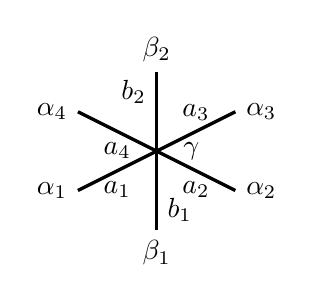
\begin{tikzpicture}[very thick]
\draw (-1, -1/2) -- (1, 1/2);
\draw (-1, 1/2) -- (1, -1/2);
\draw (0,-1) -- (0,1);
\node[right] at (1, 1/2) {$\alpha_3$};
\node[right] at (1, -1/2) {$\alpha_2$};
\node[left] at (-1, 1/2) {$\alpha_4$};
\node[left] at (-1, -1/2) {$\alpha_1$};
\node[above] at (1/2, 1/4) {$a_3$};
\node[below] at (1/2, -1/4) {$a_2$};
\node[below] at (-1/2, 1/4) {$a_4$};
\node[below] at (-1/2, -1/4) {$a_1$};
\node[above] at (0, 1) {$\beta_2$};
\node[below] at (0, -1) {$\beta_1$};
\node[left] at (0, 3/4) {$b_2$};
\node[right] at (0, -3/4) {$b_1$};
\node[right=2mm] at (0,0) {$\gamma$};
\end{tikzpicture}
\caption{A star graph $X$ which $C_4$ acts on by sending $\alpha_i\mapsto\alpha_{i+1\bmod 4}$, and by
$\beta_i\mapsto\beta_{i+1\bmod 2}$. If we think of this as coordinate axes, $C_4$ acts by rotation on the
$xy$-plane and reflection on the $z$-axis.}
\label{star_graph}
\end{figure}

Let $C_4$ act by sending $\alpha_i\mapsto\alpha_{i+1\bmod 4}$ and $\beta_i\mapsto\beta_{i+1\bmod 2}$. That is, it
reflects the $\beta$s and rotates the $\alpha$s. Hence $X$ has a $C_4$-CW structure as follows.
\begin{itemize}
	\item A single $C_4/C_4$ $0$-cell at the center $\gamma$.
	\item A single $C_4/C_2$ $0$-cell $\set{\beta_1,\beta_2}$.
	\item A single $C_4/e$ $0$-cell $\set{\alpha_1,\alpha_2,\alpha_3,\alpha_4}$.
	\item A single $C_4/C_2$ $1$-cell, which is the edges $b_1$ and $b_2$.
	\item A single $C_4/e$ $1$-cell, which is the edges $a_1,\dotsc,a_4$.
\end{itemize}
The orbit category is as in~\eqref{Cp2orbit}. Keep in mind that there are multiple maps $C_4/e\rightrightarrows
C_4/C_2$, but they're all conjugates of each other under the $C_4$-action on $C_4/e$.

To compute $\underline C_\bullet(X)$, we look at the fixed points under $\set e$, $C_2$, and $C_4$.
\begin{itemize}
	\item The fixed points under $\set e$ are of course the whole space, and so the CW chain complex is
	\[\Z\cdot\set{b_1,b_2,a_1,a_2,a_3,a_4}\longrightarrow \Z\cdot
	\set{\gamma,\beta_1,\beta_2,\alpha_1,\alpha_2,\alpha_3,\alpha_4}\]
	(seven total $0$-cells, and six total $1$-cells).
	\item The $C_2$-fixed points is the line between $\beta_1$ and $\beta_2$, so its CW chain complex is
	\[\Z\cdot\set{b_1,b_2}\longrightarrow \Z\cdot\set{\gamma, \beta_1,\beta_2}.\]
	\item The $C_4$-fixed points are just the center point, so the chain complex is $0\to\Z$.
\end{itemize}
With bases for chain groups as above, the differentials are
\[d_{C_4} = \begin{pmatrix*}[r]
	-1 & -1 & -1 & -1 & -1 & -1\\
	1 & 0\\0 & 1\\
	&& 1 & 0 & 0 & 0\\
	&&0& 1 & 0 & 0\\
	&&0&0& 1 & 0\\
	&&0&0&0& 1
\end{pmatrix*} \qquad\text{and}\qquad
d_{C_2} = \begin{pmatrix*}[r]
	-1 & -1\\
	1 & 0\\0 & 1
\end{pmatrix*},
\]
i.e.\ $\underline C_\bullet(X)$ is
\[\xymatrix{
	\ar@(dl,ul)^{C_4}\Z^7 & \Z^6\ar[l]_{d_{C_4}}\ar@(dr,ur)_{C_4}\\
	\Z^3\ar@(dl,ul)^{C_2}\ar@{^(->}[u] & \Z^2\ar@{^(->}[u]\ar[l]_{d_{C_2}}\ar@(dr,ur)_{C_2}\\
	\Z\ar@{^(->}[u] & 0.\ar[l]\ar[u]
}\]
The $C_4$-actions in the top row are the regular $C_4$-representation on the subspace generated by the $\alpha_i$
or the edges they touch. Similarly, the $C_2$-actions in the middle row are the regular representations on the
subspaces generated by the $\beta_j$ and their edges. The inclusions in the diagram $\Z^k\inj\Z^m$ are as the first
$k$ components.\index{regular representation}

Applying $\Hom(\bl,\underline\Z)$, we get the diagram
\[ \begin{tikzcd}
    \Hom_{C_4}(\Z^7, \Z) \rar["d_{C_4}^\ast" above]\dar[two heads] & \Hom_{C_4}(\Z^6, \Z)\dar[two heads] \\
    \Hom_{C_2}(\Z^3, \Z)\rar["d_{C_2}^\ast" above]\dar[two heads] & \Hom_{C_2}(\Z^2, \Z)\dar[two heads] \\
    \Hom(\Z,\Z) \rar & 0,
\end{tikzcd} \]
where the vertical arrows are given by restriction. Since the coefficient system $\underline\Z$ has trivial $C_4$ action in each entry, we have, for example, that
\begin{align*}
    \Hom_{C_4}(\Z^7, \Z) \cong \Hom(\Z^7/C_4, \Z) \cong \Hom(\Z^3,\Z) \cong \Z^3,
\end{align*}
corresponding to the orbits of $\gamma$, the $\alpha_i$'s, and the $\beta_i$'s, respectively. One may see that the diagram above is determined by what occurs on the top row, hence we get a cochain complex
\[\xymatrix{
	\Hom_{C_4}(\Z^7,\Z) \cong \Z^3\ar[r]^{\begin{psmallmatrix*}-1 & 1 & 0\\-1 & 0 & 1\end{psmallmatrix*}} & \Z^2 \cong \Hom_{C_4}(\Z^6, \Z).
}\]
So the cohomology is that of a point, which is reassuring.
\end{exm}
\begin{exm}
Let's compute Bredon cohomology with coefficients in a non-constant coefficient system. For $C_2$, this is the data
of an abelian group $A$, an involution $\vp\colon A\to A$, and a map $\Z\to A$ equivariant with respect to $\vp$.
For example, let's take $\Z[i]$ with $\vp$ acting by complex conjugation, and call this coefficient system $M$.

Let $C_2$ act on $S^2$ by reflection across a meridian $m$; this is the representation sphere $S^{1+\sigma}$. It
has a $C_2$-CW structure as follows.
\begin{itemize}
	\item One $0$-cell $e$ of the form $C_2/C_2\times D^0$ at the north pole.
	\item One $1$-cell $f$ of the form $C_2/C_2\times D^1$, which is the meridian $m$.
	\item One $2$-cell $g$ of the form $C_2/e\times D^2$, which is everything else.
\end{itemize}
For a picture, see \cref{S2CWmerid}.
\begin{figure}[h!]
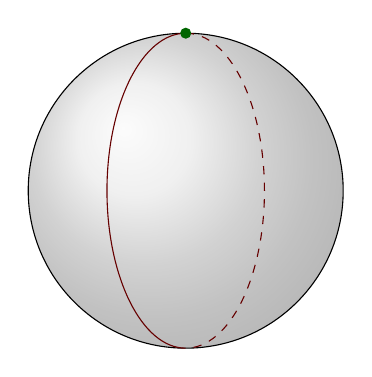
\begin{tikzpicture}
  \shade[ball color = gray!40, opacity = 0.4] (0,0) circle (2cm);
  \draw (0,0) circle (2cm);
  \draw[red!40!black] (0,2) arc (90:270:1cm and 2cm);
  \draw[dashed, red!40!black] (0,2) arc (90:-90:1cm and 2cm);
  \fill[green!40!black, fill=green!40!black] (0,2) circle (2pt);
\end{tikzpicture}
\caption{A $C_2$-CW structure for $S^{1+\sigma}$, the sphere where $C_2$ acts by reflection across a meridian.
There's a single $0$-cell $C_2/C_2\times D^0$ (the green dot), a single $1$-cell $C_2/C_2\times D^1$ (the red
circle), and a single $2$-cell $C_2/e\times D^2$ (the gray hemispheres).}
\label{S2CWmerid}
\end{figure}

Let $g_1$ and $g_2$ denote the two nonequivariant $2$-cells that make up $g$. Then, orient $f$ and $g$ such that
$\partial f = e - e = 0$ and $\partial g_1 = \partial g_2 = f$.

Then, $\underline C_\bullet(S^{1+\sigma})$ is
\[\xymatrix{
	\Z\cdot e\ar@(ul,ur)^\id & \Z\cdot f\ar@(ul,ur)^\id\ar[l]_0 & \Z\cdot\set{g_1,g_2} \ar@(ul,ur)^{\text{swap}}
	\ar[l]_-{\begin{psmallmatrix}1 & 1\end{psmallmatrix}}\\
	\Z\cdot e\ar[u]_\id & \Z\cdot f\ar[l]_0 \ar[u]_\id & 0.\ar[l]\ar[u]
}\]
Now we map to $M$. We have two copies of $\Hom(\underline\Z, M) = \Z$, and at degree $2$ we get
$\Hom_{\Z[C_2]}(\Z[C_2], \Z[i])$, which is free of rank $2$. The cochain complex is
\[\xymatrix{
	\Z\ar[r]^0 & \Z\ar[r]^{\text{rank }1} & \Z^2,
}\]
so the Bredon cohomology is
\[H_{C_2}^k(S^{1+\sigma}; M) = \begin{cases}
	\Z, &k = 0,2\\
	0, &\text{otherwise.}
\end{cases}\qedhere\]
\end{exm}

We want cohomology to have nice formal properties analogous to the Eilenberg-Steenrod axioms. We'll think of $H_G$
as a general $G$-equivariant cohomology theory of pairs $H_G^n(X, A; M)$, but in our case this will just be
$H_G^n(X/A; M)$.\index{Eilenberg-Steenrod axioms!for Bredon cohomology}
\begin{enumerate}
	\item $H_G^*$ should be invariant under weak equivalences: a weak equivalence $X\to Y$ should induce an
	isomorphism $H_G^n(Y;M) \morph^{\cong} H_G^n(X;M)$.
	\item Given a pair $A\subseteq X$, we get a long exact sequence
	\[\xymatrix{
		\dotsb\ar[r] & H_G^n(X, A; M)\ar[r] & H_G^n(X;M)\ar[r] &H_G^n(A;M)\ar[r]^-\delta &H^{n+1}(X,A;M)\ar[r] &
		\dotsb
	}\]
	\item The excision axiom: if $X = A\cup B$, then\index{excision}
	\[H_G^n(X/A; M)\cong H_G^n(B/(A\cap B); M).\]
	\item The Milnor axiom:\index{Milnor axiom}
	\[H_G^n\paren{\bigvee_i X_i; M} = \prod_i H_G^n(X_i; M).\]
	\item Finally, for now we impose the dimension axiom: our points are orbits $G/J$, so we ask that $H^n(G/H; M)$
	is concentrated in degree $0$.\index{dimension axiom}
\end{enumerate}
Some of these are easier than others: Bredon cohomology is manifestly homotopy-invariant in the same ways as
ordinary cohomology, so invariance under weak equivalence and the Milnor axiom are immediate, and excision follows
because if all spaces involved are CW complexes, $X/A\cong B/(A\cap B)$.

What takes more work is the dimension axiom and the long exact sequence. We'll show that $\underline C_n(X)$ is a
projective object, and hitting projective objects with $\Hom$ produces a long exact sequence by homological
algebra. (Recall that an object $P$ in a category where you can do homological algebra is \term{projective} if
$\Hom(P,\bl)$ is exact, which is equivalent to maps to $P$ lifting across surjections $M\surj P$.)
\begin{proof}[Proof of the dimension and long exact sequence axioms]
Observe that $\underline C_n(X)$ splits as a direct sum of pieces $H_n(G/H_+\wedge S^n)\cong \widetilde H_0(G/H)$
indexed by the cells $G/H$ of $X$. At $G/K$, $H_0(G/H) = \Z[\pi_0(G/H)^K]$. This is a free abelian group, and
we'll directly use the lifting criterion to prove this is projective. That is, we'll write down an isomorphism
\[\vp\colon\Hom_{\Fun(\sO_G\op, \Ab)}(\underline H_0(G/H), M) \morph^{\cong} M(G/H).\]
This immediately proves $\underline H_0(G/H)$ is projective: evaluating a coefficient system on an exact sequence
produces an exact sequence, and we've shown $\Hom(\underline H_0(G/H), \bl)$ is evaluation of a coefficient system.

The map $\vp$ takes a homomorphism $\theta$ and applies it to $\id_{G/H}$, which produces something in $M(G/H)$.
Why is this an isomorphism? The Yoneda lemma is a fancy answer, but you can prove it in a more elementary manner.
\begin{ex}
Calculate that any $\theta\in\Hom_{\Fun(\sO_G\op, \Ab)}(H_0(G/H), M)$ is determined by where the identity
$\id\in\Map_{\sO_G}(G/H, G/H)$ is sent, implying $\vp$ is an isomorphism.
\end{ex}
Thus, we've effectively calculated the value at $G/H$, proving the dimension axiom as well.
\end{proof}
The Eilenberg-Steenrod axioms hold for Bredon homology, and the proof is the same.
\begin{rem}
Let's foreshadow a little bit. In ordinary homotopy theory, one can show that the Eilenberg-Steenrod axioms
plus the value on points determine a cohomology theory, and this is still true in the equivariant case. But then
one wonders about Brown representability and what happens when you remove the dimension axiom --- and indeed
there are lots of interesting examples of generalized equivariant cohomology theories.
\end{rem}
\begin{ex}
We constructed a functor $\underline H\colon\Fun(\sO_G\op,\Top)\to \Fun(\sO_G\op, \Ab)$. Show that $\underline HM$
represents $H_G^n(\bl; M)$.
\end{ex}
This slick definition of $\underline H$ is one of the advantages of working with presheaves on the orbit category.
\begin{rem}
You might also want to have a universal coefficient sequence, but it's more complicated. The short exact sequence
in ordinary homotopy theory depends on the existence of short projective resolutions. Here, we have enough
projectives and injectives, but resolutions are longer. Thus, taking an injective resolution of $M$ and filtering
the resulting double complex, one obtains a spectral sequence
\[\Ext^{p,q}(\underline C_*(X), M)\Longrightarrow H_G^{p+q}(X;M).\]
{\color{red}Warning}: indexing might be slightly off.\index{universal coefficient spectral sequence}

There's a corresponding $\Tor$ spectral sequence.
\end{rem}
Since the category is more complicated, one expects to have to do more work. But sometimes there are nice results
nonetheless; Smith theory, which we discuss in the next section, is an example.
